\documentclass[a4paper, 12pt]{article}

%%% Работа с русским языком
\usepackage{cmap}					% поиск в PDF
\usepackage{mathtext} 				% русские буквы в формулах
\usepackage[T2A]{fontenc}			% кодировка
\usepackage[utf8]{inputenc}			% кодировка исходного текста
\usepackage[russian]{babel}	% локализация и переносы

%%% Дополнительная работа с математикой
\usepackage{amsmath,amsfonts,amssymb,amsthm,mathtools} % AMS
\usepackage{icomma} % "Умная" запятая: $0,2$ --- число, $0, 2$ --- перечисление

%% Номера формул
%\mathtoolsset{showonlyrefs=true} % Показывать номера только у тех формул, на которые есть \eqref{} в тексте.

%% Шрифты
\usepackage{euscript}	 % Шрифт Евклид
\usepackage{mathrsfs} % Красивый матшрифт

%% Поля
\usepackage[left=2cm,right=2cm,top=2cm,bottom=2cm,bindingoffset=0cm]{geometry}

%% Русские списки
\usepackage{enumitem}
\makeatletter
\AddEnumerateCounter{\asbuk}{\russian@alph}{щ}
\makeatother

%%% Работа с картинками
\usepackage{graphicx}  % Для вставки рисунков
\graphicspath{{images/}{images2/}}  % папки с картинками
\setlength\fboxsep{3pt} % Отступ рамки \fbox{} от рисунка
\setlength\fboxrule{1pt} % Толщина линий рамки \fbox{}
\usepackage{wrapfig} % Обтекание рисунков и таблиц текстом

%%% Работа с таблицами
\usepackage{array,tabularx,tabulary,booktabs} % Дополнительная работа с таблицами
\usepackage{longtable}  % Длинные таблицы
\usepackage{multirow} % Слияние строк в таблице

%% Красная строка
\setlength{\parindent}{2em}

%% Интервалы
\linespread{1}
\usepackage{multirow}

%% TikZ
\usepackage{tikz}
\usetikzlibrary{graphs,graphs.standard}

%% Верхний колонтитул
\usepackage{fancyhdr}
\pagestyle{fancy}

%% Перенос знаков в формулах (по Львовскому)
\newcommand*{\hm}[1]{#1\nobreak\discretionary{}
	{\hbox{$\mathsurround=0pt #1$}}{}}

%% Мои дополнения
\usepackage{float} %Добавляет возможность работы с командой [H] которая улучшает расположение на странице
\usepackage{gensymb} %Красивые градусы
\usepackage{graphicx}               % Импорт изображений
\usepackage{caption} % Пакет для подписей к рисункам, в частности, для работы caption*

% подключаем hyperref (для ссылок внутри  pdf)
\usepackage[unicode, pdftex]{hyperref}

%%% Теоремы
\theoremstyle{plain}                    % Это стиль по умолчанию, его можно не переопределять.
\renewcommand\qedsymbol{$\blacksquare$} % переопределение символа завершения доказательства

\newtheorem{theorem}{Теорема}[section] % Теорема (счетчик по секиям)
\newtheorem{proposition}{Утверждение}[section] % Утверждение (счетчик по секиям)
\newtheorem{definition}{Определение}[section] % Определение (счетчик по секиям)
\newtheorem{corollary}{Следствие}[theorem] % Следстиве (счетчик по теоремам)
\newtheorem{problem}{Задача}[section] % Задача (счетчик по секиям)
\newtheorem*{remark}{Примечание} % Примечание (можно переопределить, как Замечание)
\newtheorem{lemma}{Лемма}[section] % Лемма (счетчик по секиям)

\begin{document}
    \newcommand{\HRule}{\rule{\linewidth}{0.7mm}} % Defines a new command for the horizontal lines, change thickness here
	
	\begin{center}
		\large\textbf{Московский Физико-Технический Институт}\\ % Name of your university/college
		\large\textbf{(государственный университет)}
	
		\vfill
		
		\Large Лабораторная работа по курсу общей физики № *labnum*\\[0.5cm] % Preambule of your document title
		
		
		\HRule
		\\[0.4cm]
		{ \huge \bfseries *name of your labwork*}% Title of your document
		\\[0.4cm] 
		\HRule
		\\[0.5cm]
		
		\ \\
	\textbf{\large Автор:} \\	
	\large *your name* *groupname*\\ % Your name and something more, your group num for example
		\vfill
		\hspace*{-0.8 cm}
\includegraphics[width=100 pt]{frkt_logo}\\ % logo of your  company/university/college
		\large Долгопрудный, 2021 % location and year
	\end{center}

\newpage
\setcounter{page}{2}
\fancyfoot[c]{\thepage}
\fancyhead[L] {Работа № *labnum*} % some information in page header
\fancyhead[R]{}
    
    \textbf{Цель работы:} изучение основных принципов работы газового лазера и свойств лазерного излучения. \\
    
    \textbf{В работе использовались:} юстировочный лазер, гелий-неоновая трубка, компьютер со звуковой картой, модулятор (обтюратор), фотодиоды, зеркала, поляроид. \\
    
    \section*{Теоретическое введение}
    
    \begin{figure}
    	\centering
    	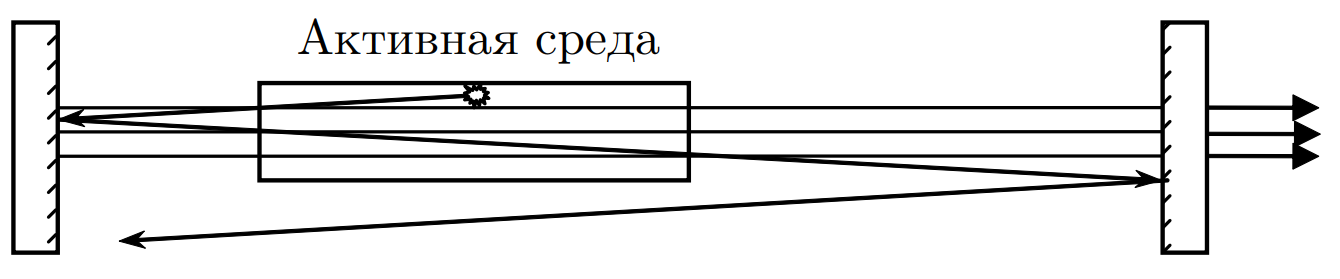
\includegraphics[scale=0.5]{Схема_лазера.png}
    	\caption{Схема лазера}
    	\label{image:scheme}
    \end{figure}
    
    Главными элементами практически любого лазера являются два параллельных друг другу зеркала и расположенная между ними среда, усиливающая свет. Усиление света основано на явлении вынужденного излучения, которое является обратным поглощению света. Как известно из опыта, при поглощении электромагнитного излучения веществом атомы или молекулы, находящиеся на каком-либо энергетическом уровне, переходят на более высокий свободный уровень, поглощая один квант (фотон) излучения. Поглощение возникает только в том случае, если энергия фотона совпадает с разницей энергий между этими уровнями. Явление вынужденного излучения заключается в том, что если атом находится на возбужденном уровне, то под действием электромагнитного поля происходит обратный переход с возбужденного уровня на более низкий уровень с излучением кванта света.
    
    Рассмотрим механизм возникновения усиления в рабочей среде гелий-неонового лазера. Лазерная трубка заполняется смесью гелия и неона в соотношении от 5:1 до 10:1 с общим давлением порядка $10^2$ Па, при котором довольно легко возбудить постоянный электрический разряд. Рабочим лазерным веществом является неон. Гелий используется для избирательного заселения верхнего рабочего уровня неона. Атомы гелия возбуждаются при столкновениях с разогнанными в электрическом поле разряда электронами. Передача энергии от возбужденных атомов гелия к атомам неона осуществляется при столкновениях между ними. Известно, что наиболее эффективно передача энергии от атома к атому происходит в резонансном случае, то есть когда энергии уровней, между которыми происходит переход, близки.
    
    \section*{Экспериментальная установка}
    
    \begin{figure}[h!]
    	\centering
    	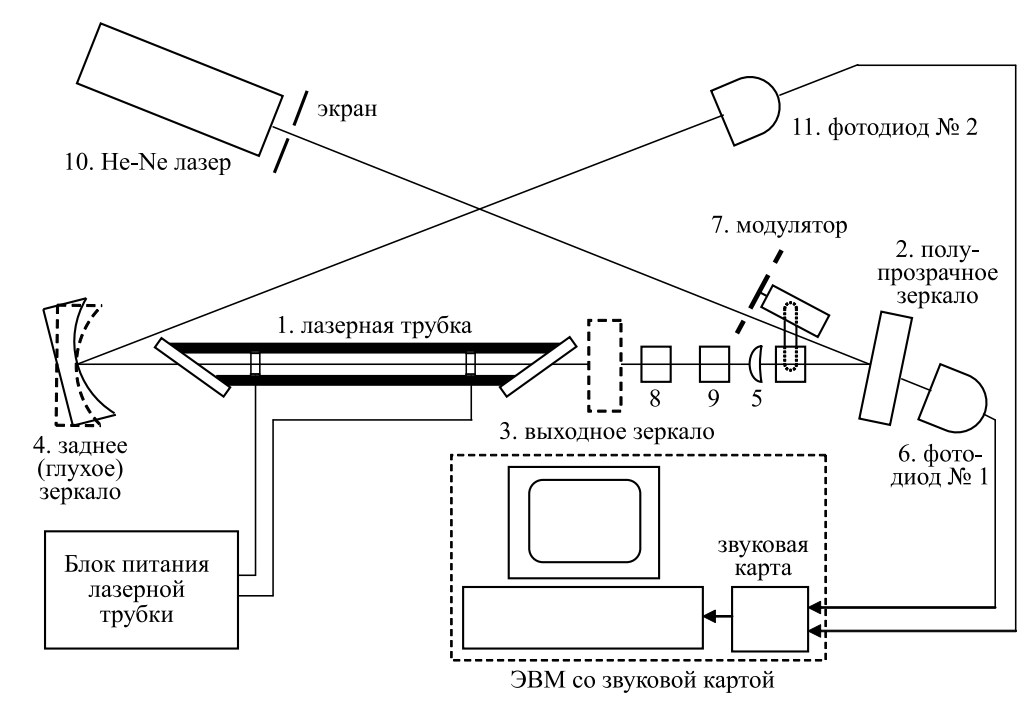
\includegraphics[scale=0.7]{images/Установка.png}
    	\caption{Экспериментальная установка}
    	\label{image:installation}
    \end{figure}
    
    Схема экспериментальной установки приведена на рис. \ref{image:installation} На оптической скамье расположены: газоразрядная трубка исследуемого He-Ne лазера ЛГ-75 (1), рейтера для крепления юстировочных оправ с зеркалами (2, 3, 4), линза, уменьшающая расходимость юстировочного лазера (5), фотодиод (6), модулятор (7) а также съемный рейтер (8) с отрицательной линзой для наблюдения модовой структуры излучения исследуемого лазера и рейтер (9), в который вставляется либо экран, либо поляроид. Юстировочный лазер (10) и фотодиод (11) закреплены на столе. Юстировочный лазер предназначен для юстировки всех элементов установки и для измерения коэффициента усиления активной среды исследуемого лазера.
    
    Поскольку коэффициент усиления на рабочей частоте лазера мал, и усиление интенсивности луча зондирующего лазера при длине трубки $\approx 1$ м составляет всего несколько процентов, в данной работе измеряется одновременно интенсивность излучения до и после прохождения исследуемой среды.

    \section*{Изучение поляризации}
    
    Закрепим в рейтере перед выходным зеркалом поляроид. Повернем и настроим фотодиод и модулятор так, чтобы пучок исследуемого лазера хорошо проходил сквозь отверстия модулятора и попадал на фотодиод. Измерим зависимость интенсивности излучения, то есть показаний компьютера, исследуемого лазера в зависимости от угла поворота поляроида. Результаты занесем в таблицу \ref{table:polarisation}:
    
    \begin{table}[h!]
    \centering
    \begin{tabular}{|c|c|c|}
    \hline
    $\theta$ & $U_{\text{эф}}$, мВ & $\sigma_U$, мВ \\ \hline
    0        & 11,9                & 0,20           \\ \hline
    20       & 18,5                & 0,50           \\ \hline
    40       & 19,8                & 0,20           \\ \hline
    60       & 17,5                & 0,10           \\ \hline
    80       & 10,4                & 0,10           \\ \hline
    100      & 3,50                & 0,02           \\ \hline
    120      & 1,90                & 0,05           \\ \hline
    140      & 2,50                & 0,03           \\ \hline
    160      & 7,30                & 0,03           \\ \hline
    180      & 14,1                & 0,30           \\ \hline
    200      & 20,5                & 0,20           \\ \hline
    220      & 20,6                & 0,20           \\ \hline
    240      & 18,8                & 0,20           \\ \hline
    260      & 11,9                & 0,10           \\ \hline
    280      & 4,30                & 0,10           \\ \hline
    300      & 1,80                & 0,10           \\ \hline
    320      & 2,50                & 0,10           \\ \hline
    340      & 7,90                & 0,10           \\ \hline
    \end{tabular}
    \caption{Зависимость интенсивности от угла поляроида}
    \label{table:polarisation}
\end{table}
    
    Построим графики зависимости напряжения и относительной интенсивности от угла поворота поляроида.
    
    \begin{figure}[h!]
    	\begin{center}
    		\begin{minipage}[h!]{0.48\linewidth}
    			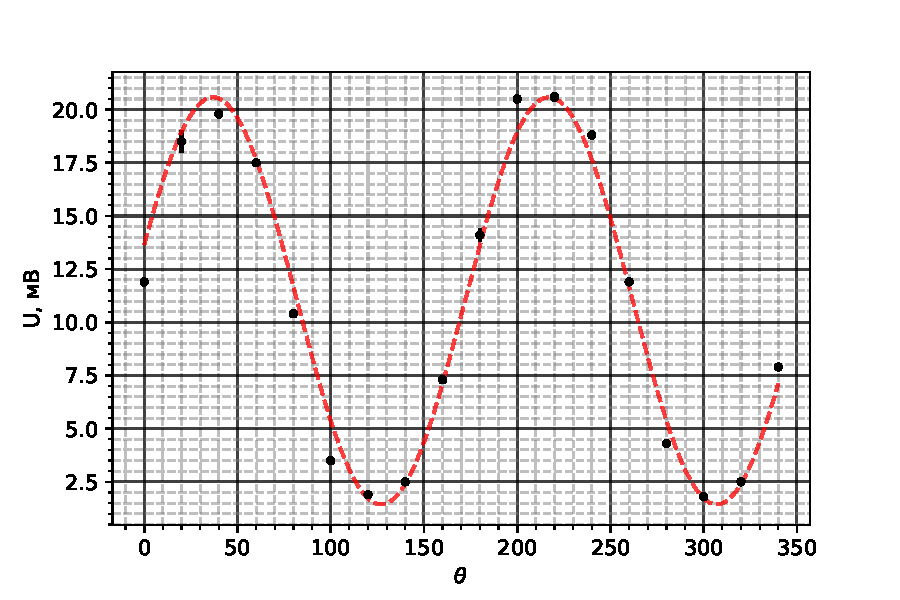
\includegraphics[width=1\linewidth]{images/polarisation.pdf}
    			\caption{График зависимости напряжения от угла поворота поляроида}
    			\label{image:polarisation}
    		\end{minipage}
    		\hfill
    		\begin{minipage}[h!]{0.48\linewidth}
    			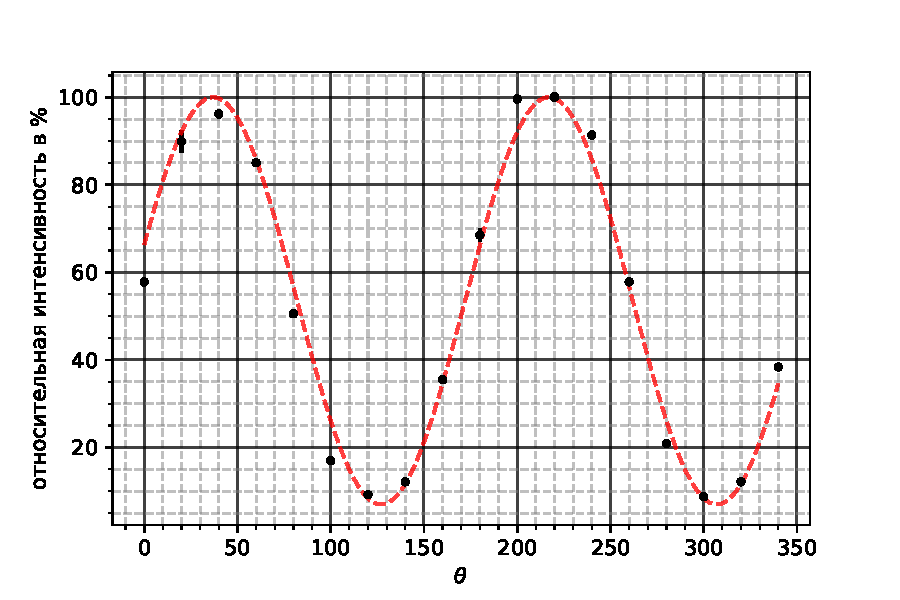
\includegraphics[width=1\linewidth]{images/relative_polarisation.pdf}
    			\caption{График зависимости относительной интенсивности от угла поворота поляроида}
    			\label{image:relative_polarisation}
    		\end{minipage}
    	\end{center}
    \end{figure}

	Наибольшее значение интенсивности лазерного излучения достигается при углах $\theta \thicksim 38 ^\circ + 180^\circ \cdot k, \; k\in \mathbb{Z}$.

	\newpage

    \section*{Наблюдение модовой структуры лазерного излучения}
    
    Пронаблюдаем строение модовой структуры лазерного излучения. Поставим на рельс вплотную к выходному зеркалу рейтер с короткофокусной линзой а в рейтер вместо поляроида вставим белый экран. Наблюдая за пятном излучения лазера, с помощью малого поворота одного зеркала получим двухмодовый, трёхмодовый и многомодовый режимы.
    
    \begin{figure}[h!]
    	\begin{center}
    		\begin{minipage}[h!]{0.48\linewidth}
    			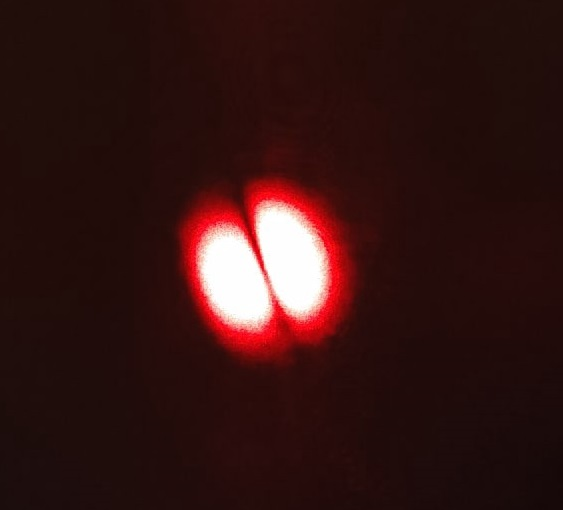
\includegraphics[width=1\linewidth]{images/Двухмодовый.jpg}
    			\caption{Наблюдение двухмодовой структуры}
    			\label{image:Two_modes}
    		\end{minipage}
    		\hfill
    		\begin{minipage}[h!]{0.48\linewidth}
    			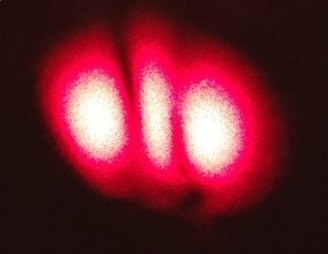
\includegraphics[width=1\linewidth]{images/Трехмодовый.jpg}
    			\caption{Наблюдение трехмодовой структуры}
    			\label{image:Three_modes}
    		\end{minipage}
    	\end{center}
    \end{figure}

	\begin{figure}[h!]
		\centering
		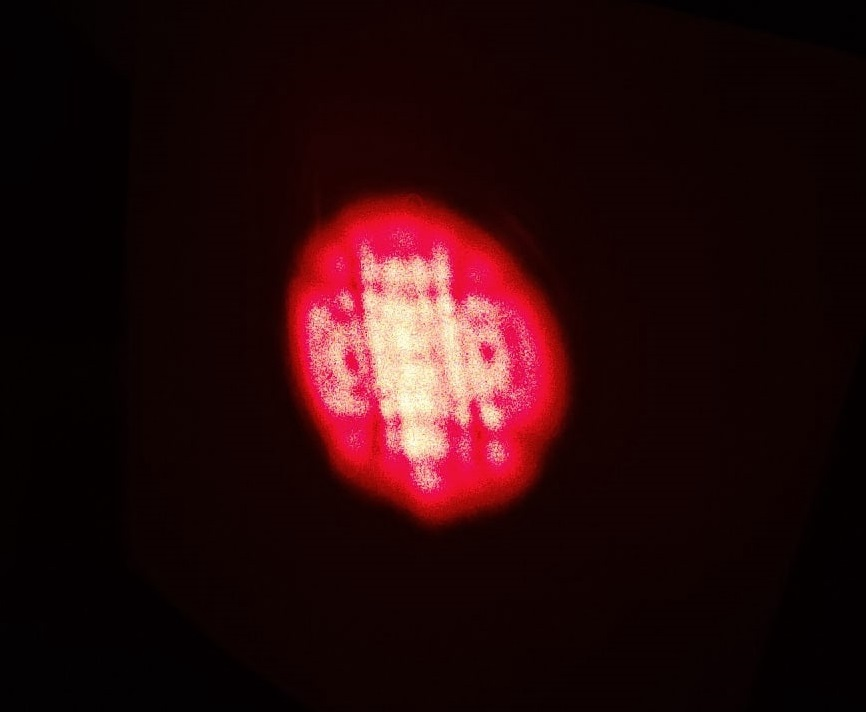
\includegraphics[scale=0.5]{images/Многомодовый.jpg}
		\caption{Наблюдение многомодовой структуры}
		\label{image:amount_modes}
	\end{figure}

	\newpage
    
    \section*{Коэффициент усиления}
    
    Включим питание исследуемого и юстировочного лазеров. Запустим осциллограф, включим режим вывода эффективных значений напряжения по обоим каналам и выберем скорость развёртки 1 мс/дел, а ее длительность -- 500 мс для наибольшей точности. Поделив отношения сигналов с  включенным и выключенным питанием трубки друг на друга, получим коэффициент усиления $G$.
    
    Выражение для коэффициента усиления:
    
    \begin{equation} \label{equation:intensity}
    	G = \frac{U_{\text{эф}}^{11}}{U_{\text{эф}}^{12}} \cdot \frac{U_{\text{эф}}^{21}}{U_{\text{эф}}^{22}}
    \end{equation}
    
    где $U_{\text{эф}}^{1i}$ -- напряжения при включенной усилительной трубке, $U_{\text{эф}}^{2i}$ -- напряжения при выключенной усилительной трубке.
    
    Вычислим погрешность коэффициента усиления по формуле:
    
    \[ \sigma_G = G \sqrt{\left(\frac{\sigma_{U^{11}}}{U^{11}} \right)^2 + \left(\frac{\sigma_{U^{12}}}{U^{12}} \right)^2 + \left(\frac{\sigma_{U^{21}}}{U^{21}} \right)^2 + \left(\frac{\sigma_{U^{22}}}{U^{22}} \right)^2} \]
    
    С выключенным питанием получаем:
    \begin{center}
    	$U_{\text{эф}}^{21} = (53,5 \pm 0,1)$ мВ \\
    	$U_{\text{эф}}^{22} = (96,0 \pm 0,2)$ мВ
    \end{center}
    
    Результаты запишем в таблицу \ref{table:intensity}.

    \begin{table}[]
    \centering
    \begin{tabular}{|c|c|c|c|c|c|c|}
    \hline
    $I$, мА & $U_1$, мВ & $\sigma_{U_1}$, мВ & $U_2$, мВ & $\sigma_{U_2}$, мВ & $G$     & $\sigma_G$ \\ \hline
    46      & 94,8      & 0,2                & 54,20     & 0,2                & 1,026   & 0,005      \\ \hline
    29      & 95,8                           & 0,3       & 55,50  & 0,2       & 1,040   & 0,006      \\ \hline
    21      & 97,3                           & 0,3       & 56,00  & 0,2       & 1,033   & 0,006      \\ \hline
    \end{tabular}
    \caption{Зависимоть коэффициента усиления от тока в трубке}
    \label{table:intensity}
\end{table}
    
    \section*{Настройка лазера на генерацию}
    
    \begin{enumerate}
    	\item Сначала настроим заднее сферическое зеркало, выходное зеркало при этом снято. Пучок, прошедший через трубку, задним зеркалом направляется строго обратно так, чтобы после вторичного прохождения через трубку исследуемого лазера он попал на экран, закреплённый на выходном торце зондирующего лазера.
    	
    	\item Поставим на скамью перед трубкой рейтер с выходным зеркалом, рабочей поверхностью к исследуемому лазеру. Это зеркало юстируем так, чтобы отраженный от него луч зондирующего лазера попал в то же самое место, куда попадал пучок, отраженный от сферического заднего зеркала.
    	
    	\item Включим блок питания исследуемого лазера. Когда загорится разряд, появляется генерация, которую мы определим по появлению ярких красных пятен на зеркалах.
    	
    	\item Тонкой подстройкой зеркал добьемся максимальной мощности генерации.
    \end{enumerate}
    
    \section*{Вывод}
    
    В данной работе мы изучили основные принципы работы газового лазера и свойства лазерного излучения на примере гелий-неонового лазера. В результате проведенной работы было установлено:
    
    \begin{enumerate}
    	\item излучение He-Ne лазера обладает **-поляризацией
    	\item пронаблюдали поперечные модовые структуры
    	\item установили коэффициент усиление среды за один проход $$G = 1,033 \pm 0,006$$
    \end{enumerate}
    
\end{document}